\chapter{Polygamy and Polyandry}

First off, let's get some definitions out of the way:

\begin{displayquote}
Polygamy: The practice or custom of having more than one wife or husband at the same 
time.
\end{displayquote}

\begin{displayquote}
Polyandry: Polygamy in which a woman has more than one husband.
\end{displayquote}

Eveyone knew Brigham Young practiced polygamy. It was thought for the longest time 
that it all began with him. Well, that's not the case. According to the LDS Church
Essay, ``Plural Marriage in Kirtland and Nauvoo"\footnote{
https://www.lds.org/topics/plural-marriage-in-kirtland-and-nauvoo?lang=eng
} we learn that Joseph Smith practed polygamy.

From the book of Jacob, we read:

\begin{displayquote}
For if I will, saith the Lord of Hosts, raise up seed unto me, 
I will command my people; otherwise they shall hearken unto these 
things.\footnote{Jacob 21:30}
\end{displayquote}

Polygamy is meant to bring up seed unto the Lord. It's a means of populating the
Earth so those people will become members of the Lord's church and continue on with
the traditions of their fathers.\footnote{Not to be confused with the vain traditions
of the wicked Lamenites.}

If that's ``one" of the reasons for practicing polygamy, why are there no offspring
of Joseph Smith from those polygmous relationships? People in the church will tell
you he married them spiritually only, but that goes against what the Book of Mormon
teaches.

Can't have it both ways, so which is it?

There are also reports of Joseph Smith marrying girls as young as 15.\footnote{
From the essay: ``The youngest was Helen Mar Kimball, daughter of Joseph’s close 
friends Heber C. and Vilate Murray Kimball, who was sealed to Joseph several 
months before her 15th birthday."
} Again, the apologetics will tell you this was normal for the time. Normal or not,
it goes against any kind of morality a person should have. I don't care the time
period in which it was normal.

Joseph was also sealed to women who were already married to other men. According to
the essay, an angel rebuked Joseph for practicing Polyandry and went back to marrying
single women.

Another moment where God forgot to specifcially announce His intentions of how
polygamy should be practiced? Again, one would think that God would have instructed
Joseph exactly in how things should be worked out. The Bible is full of examples
of the Lord telling the people exactly how to build something, why would other
principles of the gospel be any different?

Is it possible, the polygamy command didn't come from God at all? Joseph made it up
and he decided what he wanted to do and how to go about it? If that's the case,
that's not how God is meant to work. One would hope that certain commandments given
from God would have a strict understanding and expectation to be followed. A prophet
is speaking for God afterall, is he not?

Again from the same essay ``Plural Marriage in Kirtland and Nauvoo" stated above,
there is a troubling line:

\begin{displayquote}
But Emma likely did not know about all of Joseph’s sealings.
\end{displayquote}

This goes against D\&C 132.\footnote{
D\&C 132:52 And let mine handmaid, Emma Smith, receive all those that have been 
given unto my servant Joseph, and who are virtuous and pure before me; and those 
who are not pure, and have said they were pure, shall be destroyed, saith the 
Lord God.
} She was to receive all those who the Lord gave unto Joseph. if she did not know
about them, how was she to receive them? Apparently this revelation was directed
directly to Emma because she did not apporve of Joseph's polygamy practices.

There is another clause in there, if she doesn't accept Joseph's other wives, he is
exempt from the Law of Sarah and can marry other wives anyway. So even if Emma didn't
want to accept it, Joseph could go ahead and marry others as he saw fit.\footnote{
D\&C 132:65 Therefore, it shall be lawful in me, if she receive not this law, for him
to receive all things whatsoever I, the Lord his God, will give unto him, because she
did not believe and administer unto him according to my word; and she then becomes
the transgressor; and he is exempt from the law of Sarah, who administered unto
Abraham according to the law when I commanded Abraham to take Hagar to wife.
}

Polygamy came to an end in 1890 with the manifesto. Official Declaration 1 in the
LDS Scriptures. Well kinda. They had to put out a second manifesto in 1904 warning
people they would be excommunicated if they entered into plural marriage. So I guess
the first one was to say the church didn't believe in the practice, and the second
was to actually enforce the rule? I'm not quite sure.\footnote{
``The Manifesto and the End of Plural Marriage"
https://www.lds.org/topics/the-manifesto-and-the-end-of-plural-marriage?lang=eng
}

There were mixed feelings on the first manifesto to begin with, I've no idea how
people felt about the second manifesto. Not much is talked about the second manifesto
in today's church meetings. Only the first. There's a bit of things people aren't
taught about in the church, a lot of history gets glossed over; this is one of them.

In the 1835 Book of Commandments, there is an article titled Marriage. In this
article it is stated that the church only believed in monogomy. There is a little
history behind this. It is claimed by Joseph Fielding Smith that Oliver Cowdery
inserted the document ``without authority". That is to say words were put into the
1835 D\&C and the Prophet Joseph Smith did nothing to stop it.

On July 7, 1878, Joseph F. Smith talked about Oliver's writing of this article:

\begin{displayquote}
To put this matter more correctly before you, I here declare that the principle of 
plural marriage was not first revealed on the 12th day of July, 1843. It was 
written for the first time on that date, but it had been revealed to the Prophet 
many years before that, perhaps as early as 1832. About this time, or 
subsequently, Joseph, the Prophet, intrusted this fact to Oliver Cowdery; he 
abused the confidence imposed in him, and brought reproach upon himself, and 
thereby upon the church by ``running before he was sent," and "taking liberties 
without license," so to speak, hence the publication, by O. Cowdery, about this 
time, of an article on marriage, which was carefully worded, and afterwards found 
its way into the Doctrine and Covenants without authority. This article explains 
itself to those who understand the facts, and is an indisputable evidence of the 
early existence of the knowledge of the principle of patriarchal marriage by the 
Prophet Joseph, and also by Oliver Cowdery.\footnote{Joseph F. Smith, Journal of 
Discourses 20:29.}
\end{displayquote}

How is this possible that something made it into the Doctrine and Covenants without
Joesph's knowledge? It wasn't given as a revelation, it was something Oliver wrote up
himself. If that's the case? What other writings in the Doctrine and Covenants are
just the thoughts of man and not revelations?

Was Joseph Smith trying to hide polygamy from the followers of the church? It's known
that polygamy wasn't widely practiced. Considering his own wife, Emma, signed her
name on an article saying that polygamy is not practiced. She didn't know he was
marrying other women at the time or, did she know and she was lying about it?

Figure \ref{fig:tas1} shows her name and what she signed.\footnote{See Appendix D for
full article.}

\begin{figure}[h!]
  \centering
  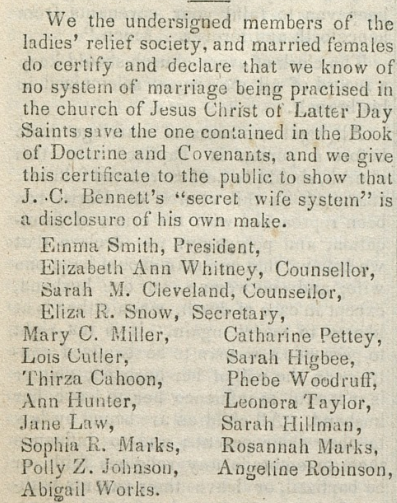
\includegraphics[width=0.4\linewidth]{articles/images/polygamy.png}
  \caption{Times and Seasons Vol 3 No. 23}
  \label{fig:tas1}
\end{figure}

The quesiton arises, at which point in time did Emma learn of plural marriage? 
Joseph began practicing plural marriage possibly as early as 1832, as mentioned by
Joseph Fielding Smith above, so it was in practice at the time Oliver published the
article in the D\&C.

Another interesting aspect of D\&C Section 132 regarding the apporval of polygamy:

\begin{displayquote}
David also received many wives and concubines, and also Solomon and Moses my 
servants, as also many others of my servants, from the beginning of creation until 
this time; and in nothing did they sin save in those things which they received 
not of me.

David’s wives and concubines were given unto him of me, by the hand of Nathan, 
my servant, and others of the prophets who had the keys of this power; and in none of 
these things did he sin against me save in the case of Uriah and his wife; and, 
therefore he hath fallen from his exaltation, and received his portion; and he 
shall not inherit them out of the world, for I gave them unto another, saith the 
Lord.\footnote{D\&C 132:38-39}
\end{displayquote}

Okay, so David had many wives and those were given to him of the Lord. So he was
commanded to have multiple wives. Yet, there is a footnote in verse 39, which points
over to the Book of Mormon:

\begin{displayquote}
But the word of God burdens me because of your grosser crimes. For behold, 
thus saith the Lord: This people begin to wax in iniquity; they understand not the 
scriptures, for they seek to excuse themselves in committing whoredoms, because of 
the things which were written concerning David, and Solomon his son.

Behold, David and Solomon truly had many wives and concubines, which thing was 
abominable before me, saith the Lord.\footnote{Jacob 2:23-24}
\end{displayquote}

Now we're learning that David's wives were an abomination before the Lord. They were
not commanded of Him. But in D\&C it says the Lord gave them to him. So, which is it
exactly? Why is there a contradiction to it all?

If Elijah restored the sealing keys of the priesthood in 1836 (April 3,
  1836)\footnote{D\&C 110} and Joseph Smith began practicing Polygamy in 1832(ish),
  how does that all work out? The timing seems to be a bit off?

Who performed the marriages between Joseph and these women? If it wasn't the sealing
power, and they were only considered as spirutal wives and not actual wives, who
performed the legal wedding ceremony in Kirtland at that time?